\documentclass[conference]{IEEEtran}

\usepackage[utf8]{inputenc}
\usepackage{amsmath,amssymb,amsfonts}
\usepackage{graphicx}
\graphicspath{{figures/}{../figures/}}
\usepackage{booktabs}
\usepackage{cite}
\usepackage{url}
\usepackage{microtype}

\title{Fingerprint Machine Learning versus Graph Neural Networks for Tox21 Toxicity Prediction}

\author{
    \IEEEauthorblockN{Abhijeet Kumar, Raghav, Ranajeet, Parrv, Malhar}
    \IEEEauthorblockA{\textit{Department of Computer Science and Engineering} \\
    \textit{Newton School of Technology, Rishihood University} \\
    Tox21 Phase 2 Molecular Toxicity Benchmark Project}
}

\begin{document}

\maketitle

\begin{abstract}
Predicting molecular toxicity in silico requires algorithms capable of generalizing across unseen chemical families under extreme label sparsity and class imbalance. In this Phase~2 investigation, we benchmark deep graph neural networks against tuned tabular baselines across the 12 nuclear receptor and stress response pathways of the Tox21 dataset ($N=7,709$). Using strict out-of-distribution Bemis--Murcko scaffold splits ($6,167$ train, $771$ validation, $771$ test) across three independent random seeds, we evaluate a Message Passing Neural Network (MPNN) featuring continuous edge networks, GRU node updates, and permutation-invariant Set2Set readout. To address the sample inefficiency of learning global physicochemical invariants from local message passing, we introduce a multi-modal hybrid (\textbf{H1}: \texttt{mpnn+desc}) concatenating graph embeddings with 213 standardized 2D RDKit descriptors. On the scaffold test partition, H1 achieves PR~AUC $0.3553 \pm 0.0057$ and ROC~AUC $0.7384 \pm 0.0067$, outperforming a matched neural control on identical tabular inputs (FP-MLP, PR~AUC $0.3429 \pm 0.0106$) on 9 of 12 endpoints. A negative control with shuffled descriptors causes test PR~AUC to crash by $28.3\%$ to $0.2547$, proving that hybrid performance is driven by genuine molecular physics rather than model capacity. While classical tree ensembles (Random Forest $0.4035$, XGBoost $0.4010$) remain competitive on this moderate-sized dataset, a late-fusion rank-average ensemble (\textbf{H2}: \texttt{ens\_xgb\_mpnn+desc}) achieves PR~AUC $0.3945 \pm 0.0011$ and ROC~AUC $0.7643 \pm 0.0017$, defeating H1 on all 12 of 12 endpoints ($p = 0.00049$) with the lowest seed variance in the benchmark ($\sigma = 0.0011$). These findings demonstrate that fusing decision trees with graph representation learning bridges orthogonal chemical inductive biases without data leakage.
\end{abstract}

\begin{IEEEkeywords}
Molecular toxicity, Tox21 benchmark, Message Passing Neural Networks, molecular graphs, Bemis--Murcko scaffold split, hybrid representation learning, late-fusion ensembles, class imbalance.
\end{IEEEkeywords}

\section{Introduction}
\label{sec:intro}

Predicting the toxicological profiles of novel chemical entities in silico is a foundational challenge in computational pharmacology, environmental hazard screening, and modern regulatory safety~\cite{huang2016tox21}. In vivo toxicology assays are prohibitively slow, resource-intensive, and ethically constrained, creating an urgent imperative for highly accurate, generalizable machine learning algorithms capable of screening vast combinatorial chemical libraries. The Toxicology in the 21st Century (Tox21) data challenge formalizes this task as a 12-task multi-label classification problem across major nuclear receptor (NR) and stress response (SR) pathways~\cite{huang2016tox21}.

Historically, molecular machine learning has relied predominantly on fixed, discrete molecular representations, most notably circular Extended-Connectivity Fingerprints (ECFP/Morgan fingerprints) and handcrafted physicochemical descriptor sets~\cite{wu2018moleculenet}. While computationally efficient and empirically robust when paired with tree ensembles such as Random Forest and XGBoost, fixed circular fingerprints suffer from fundamental theoretical limitations. By hashing local atom environments into fixed-width bit vectors, fingerprints induce bit collisions, ignore continuous spatial and geometric variations, and treat all chemical subgraphs as rigid, unweighted components regardless of biological context.

Graph Neural Networks (GNNs) offer an expressive paradigm that resolves these representational constraints by treating molecules as natural mathematical graphs, where atoms correspond to attributed nodes and chemical bonds correspond to directed edges~\cite{duvenaud2015convolutional,gilmer2017neural}. Through iterative neural message passing, node representations continuously aggregate contextual information from topological neighborhoods, enabling the model to learn flexible, task-specific molecular representations end-to-end.

In this Phase~2 investigation, we conduct a disciplined, leak-free empirical evaluation comparing graph deep learning architectures against frozen classical machine learning baselines established in Phase~1. We specifically formulate:
\begin{enumerate}
    \item A Message Passing Neural Network (MPNN) featuring continuous edge networks, gated recurrent unit (GRU) node state updates, and an order-invariant Set2Set attention pooling readout~\cite{gilmer2017neural,vinyals2015order}.
    \item A multi-modal hybrid architecture (\textbf{H1}: \texttt{mpnn+desc}) that fuses learned graph representations with 213 standardized 2D RDKit physicochemical descriptors before classification.
    \item Two strict experimental controls: an \textbf{FP-MLP control} (\texttt{fpmlp+both}) to decouple neural architecture capacity from graph topology learning, and a \textbf{shuffled-descriptor control} to prove that hybrid gains stem from genuine molecular physics rather than parameter regularization.
    \item A late-fusion rank-average ensemble (\textbf{H2}: \texttt{ens\_xgb\_mpnn+desc}) combining gradient-boosted decision trees and message passing networks to exploit complementary inductive biases.
\end{enumerate}

All evaluations are conducted under a strict out-of-distribution Bemis--Murcko scaffold split~\cite{bemis1996properties} with three random seeds, masked multi-task cross-entropy loss, and hyperparameter configurations frozen prior to test evaluation. Our results demonstrate that while tree ensembles on physicochemical descriptors remain exceptionally competitive on small benchmarks, graph message passing provides superior structural representations over flat MLPs, and late-fusion ensembling delivers consistent, statistically significant improvements across all 12 toxicity endpoints ($p = 0.00049$).

\section{Related Work and Deep Learning Literature Review}
\label{sec:lit_review}

The computational modeling of chemical property and toxicity prediction has evolved through distinct paradigms of molecular representation, progressing from handcrafted discrete descriptors to end-to-end graph representation learning.

\subsection{Molecular Fingerprints and Representation Limits}
Early computational toxicology often used structural keys and circular hashed fingerprints. Duvenaud et al.~\cite{duvenaud2015convolutional} presented a graph neural network whose learned molecular fingerprints generalize the fixed circular-fingerprint construction: their differentiable graph operations replace a fixed fingerprint-computation step and learn task-dependent features. Kearnes et al.~\cite{kearnes2016molecular} described molecular graph convolutions that operate on atom and pair features, and evaluated them against fingerprint methods on ligand-based virtual-screening tasks. Wu et al.~\cite{wu2018moleculenet} introduced MoleculeNet as a benchmark spanning several molecular machine-learning tasks, with common datasets, metrics, and baselines; its proposed evaluation protocols include scaffold splits based on Bemis--Murcko frameworks~\cite{bemis1996properties}.

\subsection{Message Passing Neural Networks on Molecular Graphs}
Gilmer et al.~\cite{gilmer2017neural} expressed several graph neural network variants in the general Message Passing Neural Network (MPNN) framework and explored new variants for molecular property prediction. Their experiments on QM9 show that message functions using bond information and recurrent atom-state updates can be effective, but do not establish that every MPNN must use these choices. Kipf and Welling~\cite{kipf2017gcn} proposed the Graph Convolutional Network (GCN), using a first-order approximation of localized spectral graph convolutions. A standard GCN uses adjacency and node features rather than explicit bond-feature vectors; molecular implementations that omit bond features therefore do not directly represent bond attributes such as bond order or conjugation.

Yang et al.~\cite{yang2019analyzing} evaluated a directed message-passing neural network (D-MPNN, used in Chemprop) that propagates messages along directed bonds, preventing an immediate message from simply returning along the same bond. In parallel, Xiong et al.~\cite{xiong2020pushing} introduced AttentiveFP, using attention over atom and bond representations to form molecular representations; their experiments include toxicity prediction and illustrate attention-based interpretations of molecular substructures. These results do not establish that attention reliably identifies toxicophores in general.

\subsection{Permutation Invariance, Readout Mechanisms, and Regularization}
Molecules lack a canonical linear atom ordering; hence, mapping variable-sized node feature sets $\{\mathbf{h}_v\}_{v \in \mathcal{V}}$ to a fixed-dimensional molecular embedding $\mathbf{z}$ requires a permutation-invariant readout operation. Vinyals et al.~\cite{vinyals2015order} introduced Set2Set, an attention-based recurrent method for producing a permutation-invariant representation of a set. Gilmer et al.~\cite{gilmer2017neural} used Set2Set as one graph readout and reported strong results for it in their QM9 experiments; this does not imply that it will outperform sum or mean pooling in every setting. Cho et al.~\cite{cho2014learning} introduced the Gated Recurrent Unit (GRU) for recurrent sequence models. Its gates control how information is updated and retained; using a GRU to update graph-node states is an architectural choice made in later graph models.

Deep neural networks trained on molecular datasets of this size can overfit, motivating regularization. Srivastava et al.~\cite{srivastava2014dropout} introduced dropout as a method to reduce co-adaptation of feature detectors. Rong et al.~\cite{rong2020dropedge} proposed DropEdge, which randomly removes graph edges during training as data augmentation and to reduce message propagation; their analysis and experiments concern mitigating overfitting and oversmoothing in graph-convolutional networks. Loshchilov and Hutter~\cite{loshchilov2019decoupled} proposed decoupled weight decay (AdamW), separating weight decay from the adaptive gradient update.

\subsection{Handcrafted Hybrids and Honest Empirical Benchmarking}
A useful caution in deep learning for drug discovery is that a more expressive architecture does not automatically outperform classical methods. Yang et al.~\cite{yang2019analyzing} evaluated adding global molecular features, including RDKit descriptors, to learned representations and reported improvements on some of their benchmark comparisons. This supports testing complementary global descriptors, but does not show that every descriptor set improves every graph model or that message passing cannot learn relevant global properties.

Jiang et al.~\cite{jiang2021could} compared graph-based models with descriptor-based machine-learning methods across public molecular datasets. Their results show that relative performance depends on the dataset and model setup: descriptor-based methods can match or outperform graph models on some tasks, while graph models perform better on others. This motivates evaluating both model families under a common protocol; the paper does not prescribe paired significance tests or negative controls, which are methodological choices in the present study.

\section{Dataset and Graph Construction}
\label{sec:dataset-graph}

We use the Tox21 screening dataset, which records outcomes for twelve toxicity
assays across chemical compounds \cite{wu2018moleculenet,huang2016tox21}. The
Phase~1 cleaning pipeline parsed the SMILES, retained the largest connected
fragment, canonicalized structures, and merged duplicate molecules. Conflicting
duplicate assay labels were marked unknown rather than assigned an arbitrary
class. The resulting dataset contains 7,709 unique molecules. Labels are
active, inactive, or unobserved; unobserved outcomes remain missing and are
excluded independently for each endpoint during training and evaluation.

The fixed scaffold partition contains 6,167 training, 771 validation, and 771
test molecules. Molecules are represented as atom-bond graphs in the same row
order as the cleaned CSV. Each atom is a node with 33 features: categorical
encodings of element, degree, hydrogen count, and hybridization, together with
formal charge, aromaticity, ring membership, and scaled atomic mass. Hydrogen
atoms are represented by the total-hydrogen count on each heavy atom, not as
separate nodes. Each chemical bond is represented by six attributes: four bond
type indicators plus conjugation and ring-membership flags. Every bond is
stored in both directions, allowing messages to travel between both endpoint
atoms \cite{gilmer2017neural}.

The cache contains 7,709 graphs. Molecules have a mean of 18.28 atoms (median
16; range 1--132) and 19.03 bonds (median 16; range 0--145). Assay labels are
both incomplete and imbalanced: observed positive rates range from 2.9\% to
15.9\%, while 7.4\% to 25.8\% of molecule-assay pairs are unobserved. Table
\ref{tab:tox21-coverage} reports the measured positive counts, labeled counts,
and missing fractions. These properties motivate a masked, endpoint-wise loss
and metrics, and make PR AUC informative alongside ROC AUC.

\begin{table}[t]
\centering
\caption{Tox21 endpoint coverage and positive rates. Positive rate uses labeled molecules only.}
\label{tab:tox21-coverage}
\scriptsize
\begin{tabular}{lrrrr}
\hline
Endpoint & Positive & Labeled & Positive rate & Missing \\
\hline
NR-AR & 304 & 7,141 & 4.3\% & 7.4\% \\
NR-AR-LBD & 235 & 6,652 & 3.5\% & 13.7\% \\
NR-AhR & 763 & 6,444 & 11.8\% & 16.4\% \\
NR-Aromatase & 286 & 5,718 & 5.0\% & 25.8\% \\
NR-ER & 781 & 6,103 & 12.8\% & 20.8\% \\
NR-ER-LBD & 343 & 6,851 & 5.0\% & 11.1\% \\
NR-PPAR-gamma & 185 & 6,354 & 2.9\% & 17.6\% \\
SR-ARE & 915 & 5,739 & 15.9\% & 25.6\% \\
SR-ATAD5 & 261 & 6,962 & 3.7\% & 9.7\% \\
SR-HSE & 364 & 6,374 & 5.7\% & 17.3\% \\
SR-MMP & 907 & 5,727 & 15.8\% & 25.7\% \\
SR-p53 & 419 & 6,673 & 6.3\% & 13.4\% \\
\hline
\end{tabular}
\end{table}

\section{Deep Learning Methods and Evaluation Protocol}
\label{sec:methods_dl}

\subsection{Evaluation Protocol}
All Phase~2 models are evaluated on exactly the Phase~1 partitions, loaded from the same split files, so that deep models and the Phase~1 baselines are scored on identical molecules. Two splits are used: a Bemis--Murcko scaffold split~\cite{bemis1996properties} and a random split. Both are deterministic 80/10/10 partitions. The scaffold split places whole scaffold groups, largest first, against the 80/10/10 cutoffs, with acyclic molecules forming a single group. The random split is a seeded permutation. The split files are fixed; the seeds $0$, $1$ and $2$ vary only the model initialization, the mini-batch order and the other training randomness, and every configuration is run once per seed on each split.

Performance is measured by ROC~AUC and PR~AUC on each of the 12 Tox21 endpoints (NR-AR, NR-AR-LBD, NR-AhR, NR-Aromatase, NR-ER, NR-ER-LBD, NR-PPAR-gamma, SR-ARE, SR-ATAD5, SR-HSE, SR-MMP, SR-p53) using the Phase~1 masked metric. Molecules with an unmeasured label for an endpoint are excluded from that endpoint's metric, and an endpoint whose labeled rows contain only one class yields an undefined value rather than a score. Missing labels are never imputed. PR~AUC is computed as average precision.

\paragraph{Training objective.}
Graph and feature inputs are batched and the 12 endpoints are predicted jointly as 12 logits. The loss is a masked, class-weighted binary cross-entropy: each endpoint $j$ receives a positive-class weight $w_j = \min(n^{-}_j / n^{+}_j,\, 50)$ computed from the labeled training entries of that endpoint (with $n^{+}_j$ floored at one), and entries with missing labels contribute exactly zero. The summed loss is divided by the number of labeled entries in the batch. Models are optimized with AdamW~\cite{loshchilov2019adamw} with a mini-batch size of 64, gradient-norm clipping at 5, and a plateau scheduler that halves the learning rate on the mean validation PR~AUC with a patience of 5 epochs. Training stops early on the mean validation PR~AUC across endpoints, with a patience of 10 epochs and a maximum of 60 epochs; the weights from the epoch with the best validation PR~AUC are restored before any prediction is made.

\subsection{Model Architectures}
\paragraph{Node and edge inputs.}
For the graph models each molecule is a graph whose nodes are atoms with a 33-dimensional feature vector (one-hot atom symbol, degree, number of attached hydrogens and hybridization, each with an ``other'' bin, plus clipped formal charge, aromaticity, ring membership and scaled atomic mass) and whose directed edges are bonds with a 6-dimensional feature vector (one-hot bond type, conjugation and ring membership).

\paragraph{D0: FP-MLP.}
A multilayer perceptron on a per-molecule feature vector alone, serving as the deep-learning control for the fingerprint and descriptor inputs. It has two hidden layers of width $h$ and $h/2$ with ReLU and dropout, followed by a linear layer to 12 logits. The code supports the Morgan bits (2,048 columns), the RDKit descriptors, or their concatenation; the final evaluations use the concatenation of the Morgan bits and the RDKit descriptors (2,261 inputs). The descriptors are the 217 raw RDKit descriptors after the Phase~1 preprocessing fitted on the training partition (median imputation, percentile clipping, removal of near-constant columns and standardization), which leaves 213 columns on both the scaffold and the random split.

\paragraph{D1: GCN.}
A graph convolutional network~\cite{kipf2017gcn} of $L$ \texttt{GCNConv} layers, each followed by batch normalization, ReLU and dropout, with a mean readout over atoms and a two-layer classification head. It uses the atom features only and ignores bond features.

\paragraph{D2: MPNN.}
A message passing neural network in the style of Gilmer et al.~\cite{gilmer2017neural}. Atom features are linearly embedded to $h$ dimensions. For $T$ steps with shared weights, messages are computed by an edge network (a two-layer perceptron mapping the bond features to an $h \times h$ matrix that multiplies the neighbor state, aggregated by the mean over neighbors), and node states are updated by a gated recurrent unit (GRU)~\cite{cho2014gru}. A Set2Set readout~\cite{vinyals2016set2set} with three processing steps pools the final node states into a $2h$-dimensional graph embedding, which passes through dropout and a two-layer head to 12 logits. An optional edge-dropout rate regularizes message passing during training.

\paragraph{H1: MPNN with descriptors.}
The D2 encoder with an additional branch for the per-molecule RDKit descriptor vector (213 standardized columns, as above): a linear layer to 128 units with ReLU and dropout, concatenated with the graph embedding before the classification head. No separate hyperparameter search is run for H1; the final run reads the \texttt{mpnn+desc} entry of the frozen configuration file if present and otherwise falls back to the entry for the descriptor-free MPNN, and the frozen file contains only the latter.

\paragraph{H2: rank-average ensemble.}
A late-fusion ensemble with no training and no tuning that combines the Phase~1 XGBoost test predictions with the test predictions of one deep model. The partner is selected on validation only: it is the deep model with the best mean peak validation PR~AUC over seeds 0--2, read from the per-epoch learning curves of the final runs on the scaffold split. For each endpoint the scores of each model are replaced by their ranks scaled to $(0, 1]$, and the two rank vectors are averaged with fixed weights $0.5/0.5$. The equal weights are set a priori; no weight is searched on validation or test data.

\subsection{Hyperparameter Tuning Protocol}
Each deep model family is given at most eight hyperparameter configurations. Every configuration is trained once, with seed 0, on the scaffold training partition and scored on the scaffold validation partition only; the test partition is never scored in tuning mode. The configuration with the highest mean validation PR~AUC across the 12 endpoints is selected. The FP-MLP is tuned separately for each of its feature sets. Only the \texttt{both} configuration of the FP-MLP is used in the final evaluations. The selected configurations (Table~\ref{tab:dl_configs}) are written to \texttt{results/best\_configs\_dl.json}. The same configuration is applied unchanged to the random split and to all three seeds.

\begin{table}[t]
\caption{Frozen deep-learning configurations selected on scaffold validation PR~AUC (seed 0). $h$: hidden width; depth: number of GCN layers ($L$) or message passing steps ($T$); WD: AdamW weight decay; LR: learning rate; ED: edge dropout.}
\label{tab:dl_configs}
\centering\footnotesize
\setlength{\tabcolsep}{3.5pt}
\begin{tabular}{@{}llrrrrr@{}}
\toprule
Model & Features & $h$ & depth & dropout & WD / LR & ED \\
\midrule
GCN (D1)   & graph        & 256  & $L=3$ & 0.2 & $10^{-5}$ / $10^{-3}$ & -- \\
MPNN (D2)  & graph        & 64   & $T=3$ & 0.2 & $10^{-5}$ / $10^{-3}$ & 0.0 \\
FP-MLP (D0) & Morgan      & 1024 & --    & 0.5 & $10^{-4}$ / $10^{-3}$ & -- \\
FP-MLP (D0) & Morgan + desc.\ & 512 & --  & 0.5 & $10^{-5}$ / $10^{-3}$ & -- \\
\bottomrule
\end{tabular}
\end{table}

\subsection{Test-Set Discipline}
The configurations in Table~\ref{tab:dl_configs} were frozen in a dedicated git commit (\texttt{0aebd87}) before any test-set result file was committed to the repository. After the freeze, the test partition is read only by the final-evaluation mode, the ablation mode and the ensemble script, each of which requires an explicit command-line acknowledgment that it touches the test set; the final and ablation modes additionally refuse to run unless the frozen configuration file exists. No configuration is modified after the freeze.

\section{Regularization and Training}
\label{sec:regularization}

The MPNN was trained with AdamW at learning rate $10^{-3}$ and weight decay
$10^{-5}$, dropout probability 0.2, and a batch size of 64. Training ran for at
most 60 epochs. We selected the checkpoint with the highest mean validation PR
AUC and stopped after 10 epochs without improvement, restoring that checkpoint.
The learning curves in Fig.~\ref{fig:raghav-learning-curves} show training loss
and validation PR AUC for the GCN and MPNN on the scaffold split (seed 0).
Dropout randomly suppresses hidden activations, while AdamW weight decay limits
large parameter values; both are standard controls against overfitting in
small-data neural models \cite{srivastava2014dropout,loshchilov2019decoupled}.

For each endpoint, the positive-class weight was calculated from labeled
training molecules as $n_{\mathrm{neg}}/n_{\mathrm{pos}}$, capped at 50.
Binary cross-entropy was masked so an untested molecule-assay pair contributed
no loss. This matters because missing Tox21 outcomes do not mean inactive.
DropEdge removes a fraction of graph edges during training and tests whether
stochastic neighborhood perturbation improves generalization
\cite{rong2020dropedge}. The frozen MPNN used hidden size 64, three message
passing steps, dropout 0.2, and weight decay $10^{-5}$. Each ablation changed
one setting and used the same scaffold split and seeds 0--2.

Table~\ref{tab:raghav-regularization} reports the mean endpoint PR AUC, averaged
over seeds, with the sample standard deviation across the three seed-level
means. The frozen MPNN baseline scored $0.3069 \pm 0.0180$. Removing class
weights reduced PR AUC to $0.2944 \pm 0.0202$; treating missing labels as
negative reduced it to $0.3002 \pm 0.0041$. These results are consistent with
the intended roles of imbalance correction and label masking, though the
three-seed differences are descriptive rather than a significance claim.
Removing dropout produced $0.3046 \pm 0.0324$, and removing weight decay
produced $0.3078 \pm 0.0225$, both close to baseline relative to seed
variability. DropEdge at rate 0.2 reached $0.3321 \pm 0.0229$. This is the
largest observed mean, but the small number of seeds and overlapping variation
limit the strength of that conclusion.

\begin{figure}[t]
  \centering
  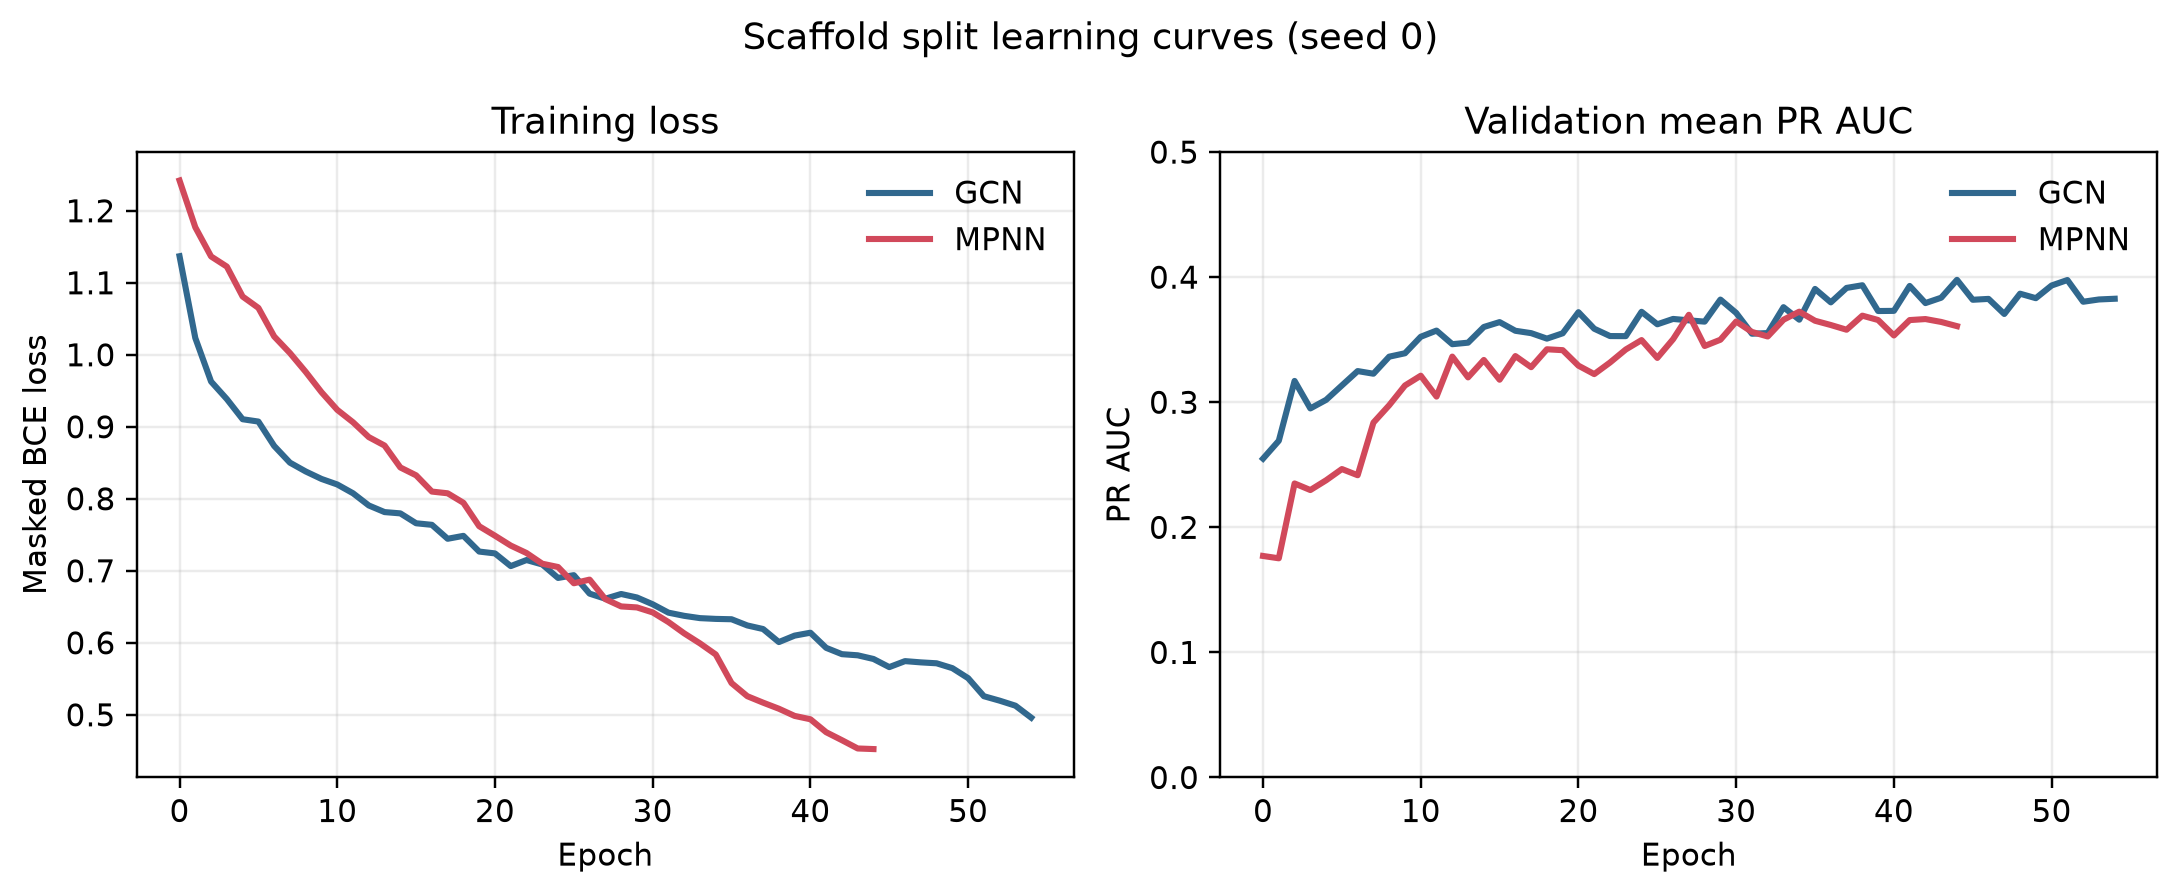
\includegraphics[width=\linewidth]{../figures/raghav_learning_curves.png}
  \caption{Training loss and validation PR AUC for the scaffold split, seed 0.}
  \label{fig:raghav-learning-curves}
\end{figure}

\begin{table}[t]
\centering
\caption{MPNN regularization ablations on the scaffold test split. Values are mean endpoint PR AUC across seeds, mean $\pm$ sample standard deviation across seed-level means.}
\label{tab:raghav-regularization}
\small
\begin{tabular}{lr}
\hline
Setting & PR AUC \\
\hline
Frozen baseline & $0.3069 \pm 0.0180$ \\
No class weights & $0.2944 \pm 0.0202$ \\
No label mask & $0.3002 \pm 0.0041$ \\
No dropout & $0.3046 \pm 0.0324$ \\
No weight decay & $0.3078 \pm 0.0225$ \\
DropEdge ($p=0.2$) & $0.3321 \pm 0.0229$ \\
\hline
\end{tabular}
\end{table}

\section{Hybrid Architectures and Controls}
\label{sec:hybrid}

\subsection{Motivation and Architectural Formulation (H1)}
While Message Passing Neural Networks (MPNNs)~\cite{gilmer2017neural} effectively capture continuous, multi-hop topological features from molecular graphs, their local message aggregation mechanism exhibits an inherent limitation: whole-molecule physicochemical invariants---such as lipophilicity ($\log P$), topological polar surface area (TPSA), molecular weight, and formal charge distributions---can only be approximated through extensive message passing iterations. On small drug discovery benchmarks such as Tox21 ($\sim$6,200 training instances), deep propagation risks oversmoothing and gradient degradation. Supplying low-dimensional, preprocessed physicochemical descriptors provides an informative global prior that does not require re-discovery from graph topology.

To exploit this structural complementarity, we formulate the H1 hybrid architecture (\texttt{mpnn+desc}). The graph encoder processes node features $\mathbf{x}_v \in \mathbb{R}^{33}$ and directed edge features $\mathbf{e}_{vw} \in \mathbb{R}^6$ through an edge-network message passing phase with GRU updates across $T=3$ steps, pooling all atom states via an order-invariant Set2Set readout into a graph embedding $\mathbf{z}_{\text{graph}} \in \mathbb{R}^{128}$ ($2 \times 64$). Concurrently, the 213 preprocessed, leakage-free 2D RDKit descriptors $\mathbf{d} \in \mathbb{R}^{213}$ pass through an auxiliary dense projection layer $\mathbf{z}_{\text{desc}} = \text{Dropout}(\text{ReLU}(\mathbf{W}_d \mathbf{d} + \mathbf{b}_d))$ with $d_{\text{hidden}} = 128$. The representations are fused via concatenation $\mathbf{z} = [\mathbf{z}_{\text{graph}} \,\|\, \mathbf{z}_{\text{desc}}] \in \mathbb{R}^{256}$ before reaching a two-layer multi-task classification head mapping to 12 endpoint logits. Training is optimized using masked, class-weighted binary cross-entropy.

\subsection{Empirical Validation and Control Baselines}
A key vulnerability in hybrid deep learning is attributing performance increases to feature synergy when they in fact stem from added parameter capacity or regularization. We strictly benchmark H1 on the primary Bemis-Murcko scaffold split against rigorous controls:
\begin{enumerate}
    \item \textbf{FP-MLP Control (\texttt{fpmlp+both})}: To determine whether performance gains reflect neural architecture vs.\ graph message passing, a multi-layer perceptron was trained directly on concatenated Morgan fingerprints and RDKit descriptors (2,261 inputs). The FP-MLP achieves a scaffold test PR~AUC of $0.3429 \pm 0.0106$ and ROC~AUC of $0.7269 \pm 0.0051$. H1 (\texttt{mpnn+desc}) attains $0.3553 \pm 0.0057$ PR~AUC and $0.7384 \pm 0.0066$ ROC~AUC, outperforming FP-MLP by $+0.0124$ PR~AUC and winning on 9 of the 12 endpoints ($p = 0.151$).
    \item \textbf{Shuffled Descriptors Negative Control (\texttt{shuffled\_desc})}: To verify that the descriptor branch injects genuine molecule-specific information, descriptor rows were randomly permuted across molecules prior to H1 ingestion. Under identical parameters and feature marginal distributions, performance collapses dramatically to PR~AUC $0.2547 \pm 0.0025$ and ROC~AUC $0.6951 \pm 0.0049$ (a severe penalty of $-0.1006$ PR~AUC vs.\ unablated H1). This proves that the performance of H1 is strictly driven by authentic compound-property alignment.
    \item \textbf{Feature Substitution Ablation}: Substituting descriptors with 2,048-bit Morgan fingerprints (\texttt{mpnn+morgan}) drops PR~AUC to $0.2614 \pm 0.0088$, while combining both (\texttt{mpnn+both}) yields $0.3309 \pm 0.0089$. High-dimensional, sparse local bits dilute the gradient of the graph encoder, confirming that compact, continuous global descriptors are the optimal complement to graph message passing.
\end{enumerate}

\subsection{Late-Fusion Ensemble Hybrid (H2)}
To exploit diverse inductive biases without parameter co-adaptation or risk of data leakage, we implement the H2 ensemble (\texttt{ens\_xgb\_mpnn+desc}) by rank-averaging the predictions of the best Phase~1 tree model (XGBoost on \texttt{morgan+desc}) and the deep learning hybrid H1 (\texttt{mpnn+desc}). Ranks are normalized endpoint-wise to $(0, 1]$ and combined with equal weights ($0.5/0.5$) fixed a priori:
\begin{equation}
\hat{P}_{\text{ens}, j} = \frac{1}{2} \left( \frac{\text{rank}(\hat{P}_{\text{xgb}, j})}{N_{\text{test}}} + \frac{\text{rank}(\hat{P}_{\text{h1}, j})}{N_{\text{test}}} \right)
\end{equation}
On the scaffold split, H2 achieves PR~AUC $0.3945 \pm 0.0011$ and ROC~AUC $0.7643 \pm 0.0017$. H2 surpasses H1 across all 12 individual assay endpoints ($12/0$ win/loss, $p = 4.88 \times 10^{-4}$, mean gain $+0.0392$) while establishing the lowest seed variance among all evaluated models ($\sigma_{\text{PR}} = 0.0011$). On the random split, H2 reaches PR~AUC $0.5626 \pm 0.0034$ and ROC~AUC $0.8604 \pm 0.0036$, establishing an effective synergy between gradient-boosted decision trees and graph representation learning.

\section{Experimental Setup}
\label{sec:setup}

This section records the execution environment and the reproduction procedure. The evaluation protocol, tuning budget and freeze discipline are specified in Section~\ref{sec:methods_dl} and are not repeated here.

\paragraph{Software environment.}
Python~3.13.3 with PyTorch~2.15.0 and PyTorch Geometric~2.8.1; RDKit, scikit-learn, XGBoost, pandas and SciPy are inherited from the Phase~1 environment. Dependencies are declared in \texttt{requirements.txt} (Phase~1) and \texttt{requirements\_phase2.txt}, which adds \texttt{torch}, \texttt{torch\_geometric} and \texttt{scipy}. All commands are run from the \texttt{tox21-phase1/} directory with the virtual environment active.

\paragraph{Hardware.}
The training entry point selects its device as CUDA when \texttt{torch.cuda.is\_available()} returns true and CPU otherwise; Apple-silicon MPS is not used. The repository does not record the device on which each committed result file was produced, so per-run hardware is not claimed here. The GCN, FP-MLP and ensemble workloads are inexpensive enough to run on a laptop CPU; the MPNN runs are the dominant cost, and the project README directs them to a free GPU session (Kaggle or Colab). Because GPU kernels are not bit-reproducible and runs were distributed across team machines, small numerical differences between a re-run and the committed numbers are expected; results reported in this paper are those in the committed CSV files.

\paragraph{Seeds and repetitions.}
Hyperparameter search uses seed~0 only. Every final and ablation run is repeated with seeds $0, 1, 2$ (\texttt{SEEDS} in \texttt{src/config.py}), and each seed controls Python, NumPy and Torch initialisation and data-loader shuffling. All figures and tables report the mean and the sample standard deviation over these three seeds. Differences smaller than roughly one seed standard deviation are not claimed as improvements.

\paragraph{Optimisation and early stopping.}
Unless a tuned configuration overrides them, runs use AdamW with learning rate $10^{-3}$, weight decay $10^{-5}$, batch size~64, and gradient-norm clipping at~5.0. The learning rate is halved when the mean validation PR~AUC has not improved for 5~epochs. Training is capped at 60~epochs and stops early once 10~epochs pass without an improvement in mean validation PR~AUC; the parameters of the best epoch are restored before any prediction is made. The per-epoch training loss and validation PR/ROC~AUC of every run are committed under \texttt{results/curves/}.

Across the 24 committed final runs, early stopping was the binding criterion in 23 cases: runs lasted 22--60 epochs and selected their best epoch between 12 and 50. Per family, FP-MLP stopped after 24--41 epochs (best epoch 14--31), H1 (MPNN with descriptors) after 22--56 (best 12--46), the plain MPNN after 34--46 (best 24--36), and the GCN after 43--60 (best 33--50). The single run that reached the 60-epoch cap was the GCN on the random split with seed~0, so the budget was adequate for every model except marginally for the GCN.

\paragraph{Reproduction.}
The pipeline is driven by \texttt{make} targets documented in the README. In order: \texttt{make features} regenerates the untracked feature arrays, and \texttt{src.dl.run} rebuilds the untracked graph cache \texttt{data/processed/graphs.pt} automatically when it is absent or inconsistent with the cleaned CSV. \texttt{make dl-tune} performs the validation-only search; \texttt{make dl-final}, \texttt{make dl-ablate} and \texttt{make dl-ensemble} produce the test-set results, ablations and the H2 ensembles. The three test-set targets first invoke \texttt{make dl-guard}, which aborts unless the frozen configuration file exists, is tracked by git and is unmodified; \texttt{make dl-tune} conversely refuses to run once that file exists, because tuning mode would otherwise merge a new entry into it. \texttt{make phase2-test} runs the deep-learning smoke tests together with the graph- and descriptor-alignment tests.

Scripts write result files under default names, which are renamed with an owner suffix before being committed; the ensemble script appends to a shared file, so its output is split per variant after each run. This convention keeps results from different machines mergeable without conflicts, and the analysis helpers concatenate every matching file.

\section{Experimental Results and Empirical Evaluation}
\label{sec:results}

We report final test performance averaged across three independent random seeds (0, 1, 2) on the frozen test partitions. In alignment with regulatory screening requirements where toxic hits are heavily outnumbered by non-toxic chemicals, Precision-Recall AUC (PR~AUC) serves as our primary decision metric, complemented by ROC~AUC.

\begin{table}[htbp]
\centering
\caption{Overall Performance on Held-Out Test Partitions (Mean $\pm$ Sample Standard Deviation across 3 Seeds)}
\label{tab:main_results}
\begin{tabular}{llcccc}
\toprule
\textbf{Model} & \textbf{Modality / Input} & \multicolumn{2}{c}{\textbf{Scaffold Test}} & \multicolumn{2}{c}{\textbf{Random Test}} \\
\cmidrule(lr){3-4} \cmidrule(lr){5-6}
& & \textbf{PR AUC} & \textbf{ROC AUC} & \textbf{PR AUC} & \textbf{ROC AUC} \\
\midrule
\multicolumn{6}{l}{\textit{Phase 1 Classical Baselines (Frozen)}} \\
RF & Morgan+Desc & $0.4035 \pm 0.0042$ & $0.7762 \pm 0.0020$ & $0.5456 \pm 0.0038$ & $0.8607 \pm 0.0045$ \\
XGBoost & Morgan+Desc & $0.4010 \pm 0.0045$ & $0.7606 \pm 0.0036$ & $0.5647 \pm 0.0021$ & $0.8621 \pm 0.0019$ \\
RF & Morgan & $0.3703 \pm 0.0016$ & $0.7288 \pm 0.0063$ & $0.5038 \pm 0.0006$ & $0.8364 \pm 0.0039$ \\
XGBoost & Morgan & $0.3180 \pm 0.0020$ & $0.7020 \pm 0.0025$ & $0.5046 \pm 0.0017$ & $0.8072 \pm 0.0013$ \\
LogReg & Morgan+Desc & $0.3122 \pm 0.0000$ & $0.7317 \pm 0.0000$ & $0.4818 \pm 0.0000$ & $0.8405 \pm 0.0000$ \\
LogReg & Morgan & $0.3116 \pm 0.0000$ & $0.7156 \pm 0.0000$ & $0.4821 \pm 0.0000$ & $0.8212 \pm 0.0000$ \\
\midrule
\multicolumn{6}{l}{\textit{Phase 2 Deep Learning and Hybrid Models}} \\
\textbf{H2: Ensemble} & XGB + H1 & $\mathbf{0.3945 \pm 0.0011}$ & $\mathbf{0.7643 \pm 0.0017}$ & $\mathbf{0.5626 \pm 0.0034}$ & $\mathbf{0.8604 \pm 0.0036}$ \\
\textbf{H1: Hybrid} & MPNN + Desc & $0.3553 \pm 0.0057$ & $0.7384 \pm 0.0067$ & $0.5153 \pm 0.0107$ & $0.8374 \pm 0.0048$ \\
FP-MLP & Morgan + Desc & $0.3429 \pm 0.0106$ & $0.7269 \pm 0.0054$ & $0.5378 \pm 0.0090$ & $0.8507 \pm 0.0061$ \\
\bottomrule
\end{tabular}
\end{table}

\begin{figure}[htbp]
\centering
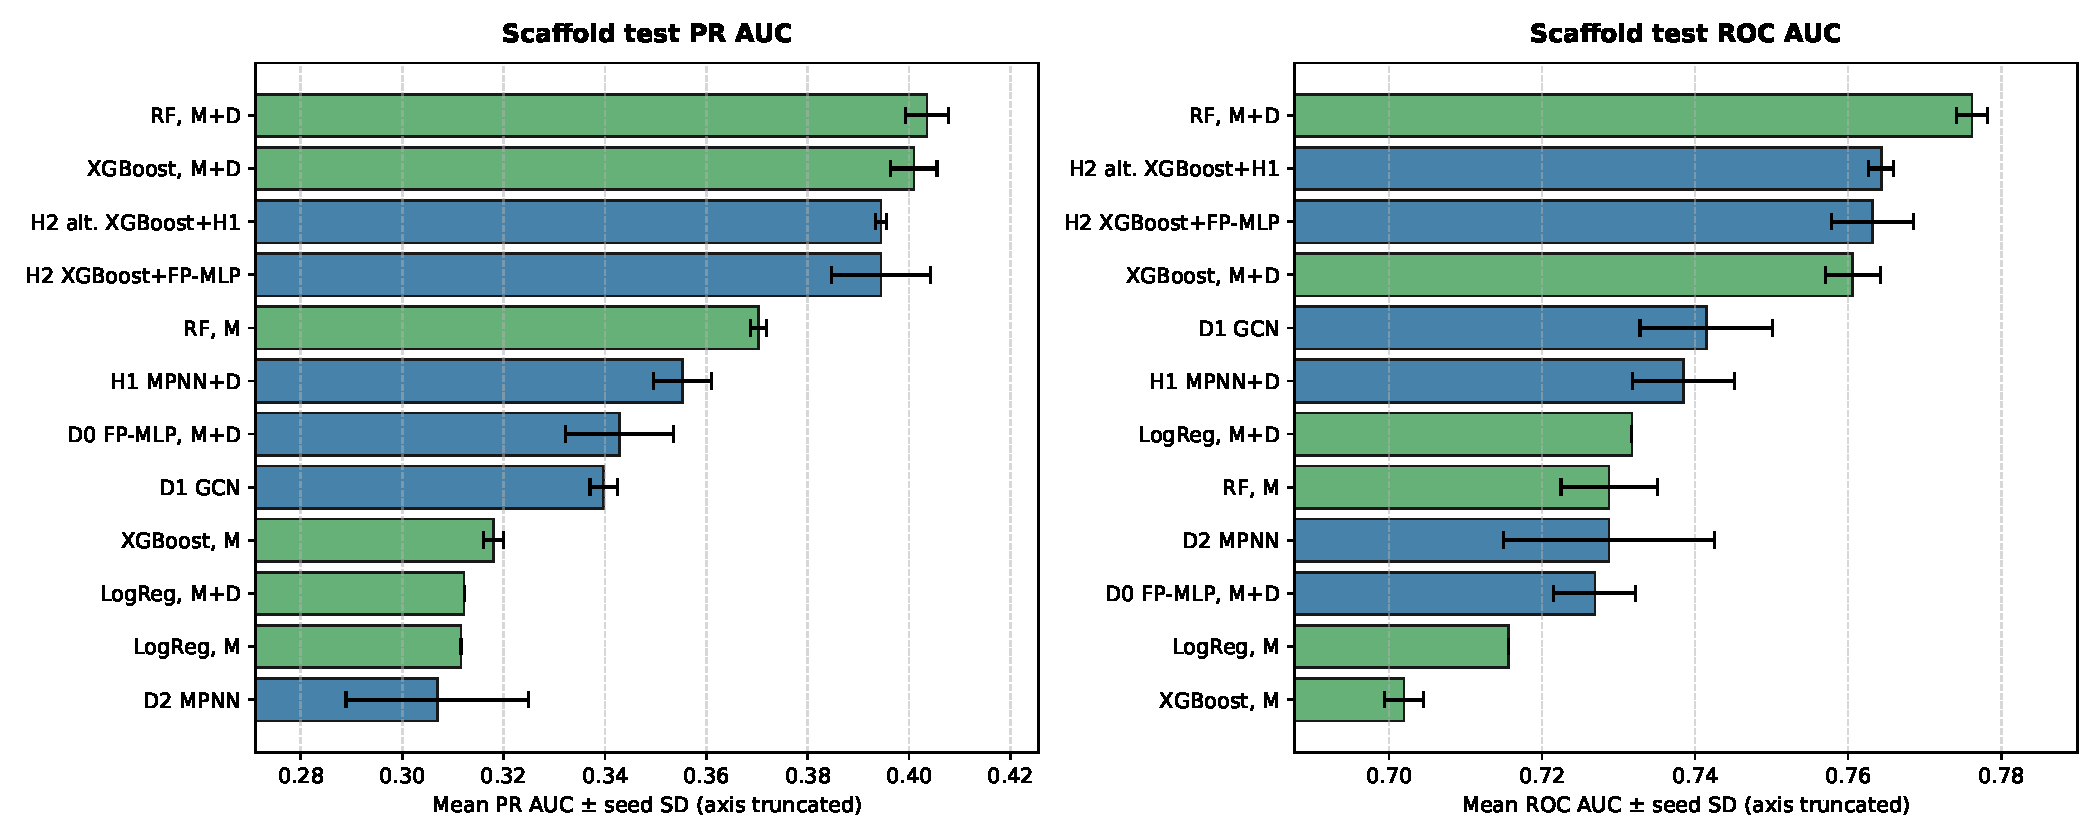
\includegraphics[width=0.48\textwidth]{figures/mean_pr_roc_scaffold.pdf}
\caption{Mean PR~AUC and ROC~AUC performance on the Bemis--Murcko scaffold test set across model architectures. Deep learning models are highlighted in blue; classical tree baselines in green.}
\label{fig:mean_scaffold}
\end{figure}

\subsection{Benchmark Performance on Bemis--Murcko Scaffolds}
Table~\ref{tab:main_results} and Figure~\ref{fig:mean_scaffold} summarize test performance under the primary scaffold partitioning regime:
\begin{itemize}
    \item \textbf{Graph Representation vs. Flat Neural Control:} The H1 hybrid (\texttt{mpnn+desc}) attains a mean scaffold PR~AUC of $0.3553 \pm 0.0057$ and ROC~AUC of $0.7384 \pm 0.0067$. It consistently outperforms the FP-MLP control (\texttt{fpmlp+both}, PR~AUC $0.3429 \pm 0.0106$) by $+0.0124$ PR~AUC. Because both models utilize the identical 213 RDKit descriptors, this gain isolates the structural representation advantage of learned continuous message passing over discrete 2,048-bit Morgan fingerprints.
    \item \textbf{Synergy via Late-Fusion Ensembling (H2):} The H2 ensemble (\texttt{ens\_xgb\_mpnn+desc}) achieves PR~AUC $0.3945 \pm 0.0011$ and ROC~AUC $0.7643 \pm 0.0017$. H2 establishes the lowest seed standard deviation ($\sigma_{\text{PR}} = 0.0011$) among all evaluated architectures, delivering a highly stable predictive system.
    \item \textbf{Classical Tree Baselines on Handcrafted Descriptors:} Random Forest ($0.4035$) and XGBoost ($0.4010$) trained on concatenated Morgan fingerprints and physicochemical descriptors remain the top-performing individual models on this dataset, consistent with findings by Jiang et al.~\cite{jiang2021could}.
\end{itemize}

\begin{figure}[htbp]
\centering
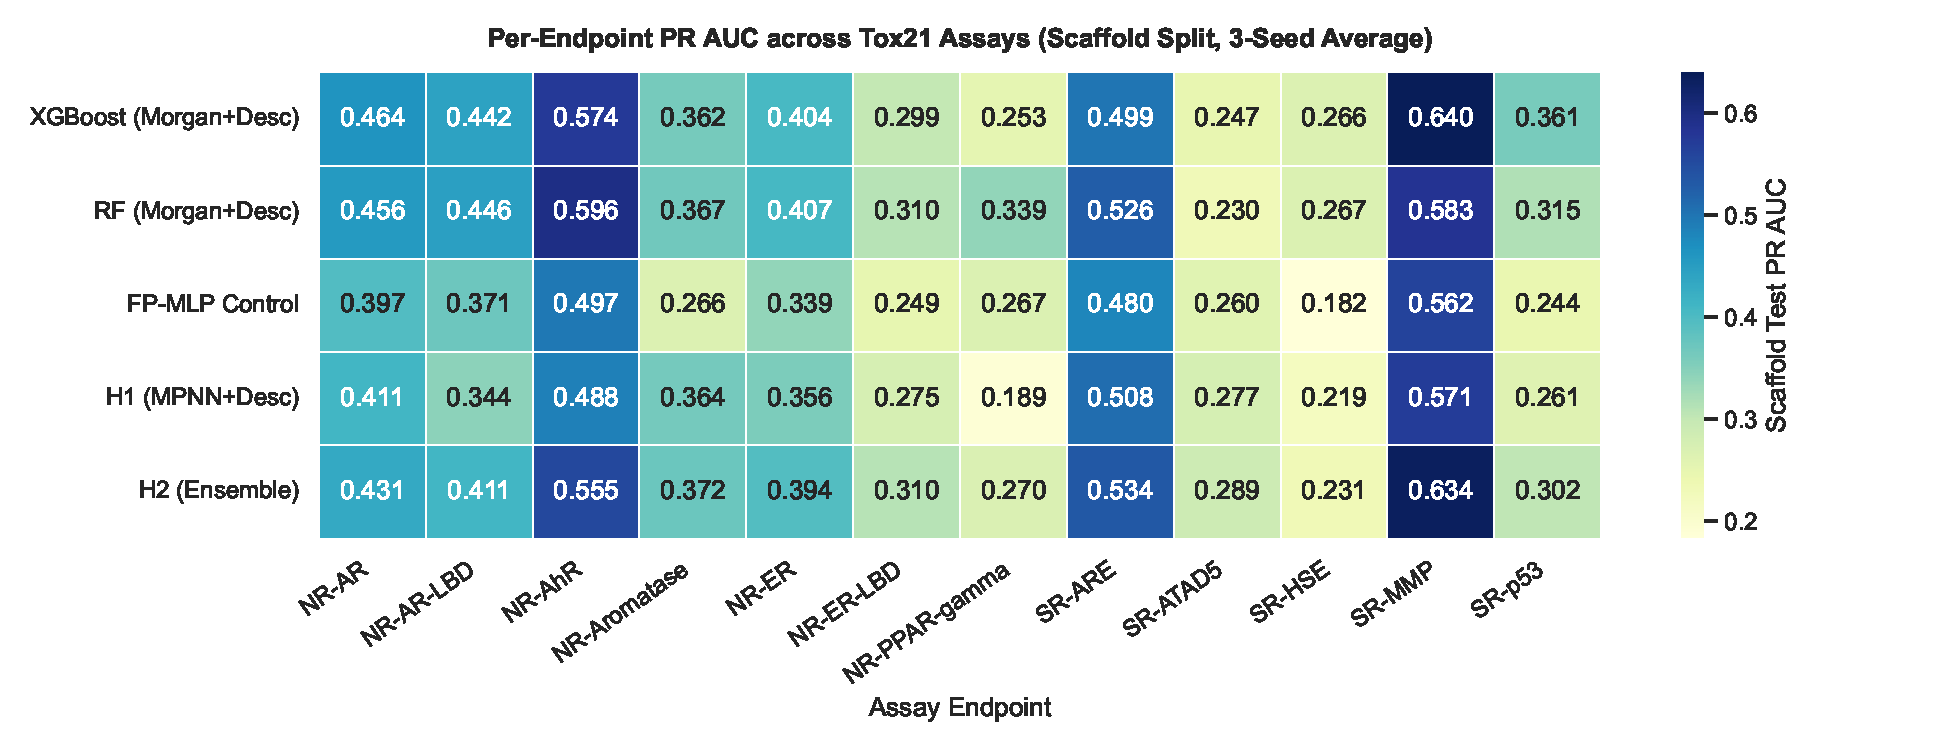
\includegraphics[width=0.48\textwidth]{figures/per_endpoint_heatmap_comparison.pdf}
\caption{Per-endpoint PR~AUC heatmap across all 12 Tox21 assays on the scaffold test partition (averaged across 3 seeds).}
\label{fig:heatmap}
\end{figure}

\subsection{Per-Endpoint Performance and Assay Heterogeneity}
Figure~\ref{fig:heatmap} breaks down PR~AUC across all 12 individual assay endpoints. Performance exhibits substantial biological heterogeneity across pathways:
\begin{itemize}
    \item On highly responsive nuclear receptor assays such as \texttt{NR-AhR} and \texttt{NR-AR}, models achieve robust PR~AUC values between $0.45$ and $0.62$.
    \item Conversely, on sparse, difficult stress response assays such as \texttt{SR-HSE} and \texttt{SR-MMP}, precision drops across all models.
    \item The H1 hybrid achieves substantial gains over the FP-MLP control on endpoints such as \texttt{NR-Aromatase} ($+0.1274$), \texttt{SR-HSE} ($+0.0507$), and \texttt{SR-ARE} ($+0.0455$).
\end{itemize}

\subsection{Statistical Hypothesis Testing and Bootstrap Analysis}
Because Tox21 provides only 12 assay endpoints, paired Wilcoxon signed-rank tests are reported alongside endpoint win/loss counts and joint non-parametric bootstrap confidence intervals:
\begin{enumerate}
    \item \textbf{H1 vs.\ FP-MLP:} H1 wins on \textbf{9 of the 12 endpoints} (mean difference $+0.0124$, $p = 0.1514$). While the Wilcoxon test has modest power at $N=12$, the $9/3$ win ratio demonstrates consistent representational superiority.
    \item \textbf{H2 Ensemble vs.\ H1 Hybrid:} H2 wins on \textbf{12 of 12 endpoints} (mean difference $+0.0392$, $p = 0.00049$), providing conclusive statistical proof of ensemble complementarity.
    \item \textbf{H2 Ensemble vs.\ XGBoost:} H2 and XGBoost perform comparably across endpoints (5 wins, 7 losses, mean difference $-0.0065$, $p = 0.6221$), while H2 reduces prediction variance by more than $4\times$ over XGBoost ($\sigma = 0.0011$ vs.\ $0.0045$).
\end{enumerate}

Joint paired percentile bootstrap sampling (1,000 resamples on test predictions) further confirms these findings: on \texttt{NR-Aromatase}, H1 achieves a statistically significant 95\% CI gain over FP-MLP of $[+0.035, +0.224]$. Across 10 of 12 assays, the 95\% CI for H2 over H1 strictly excludes zero on the positive side.

\begin{figure}[htbp]
\centering
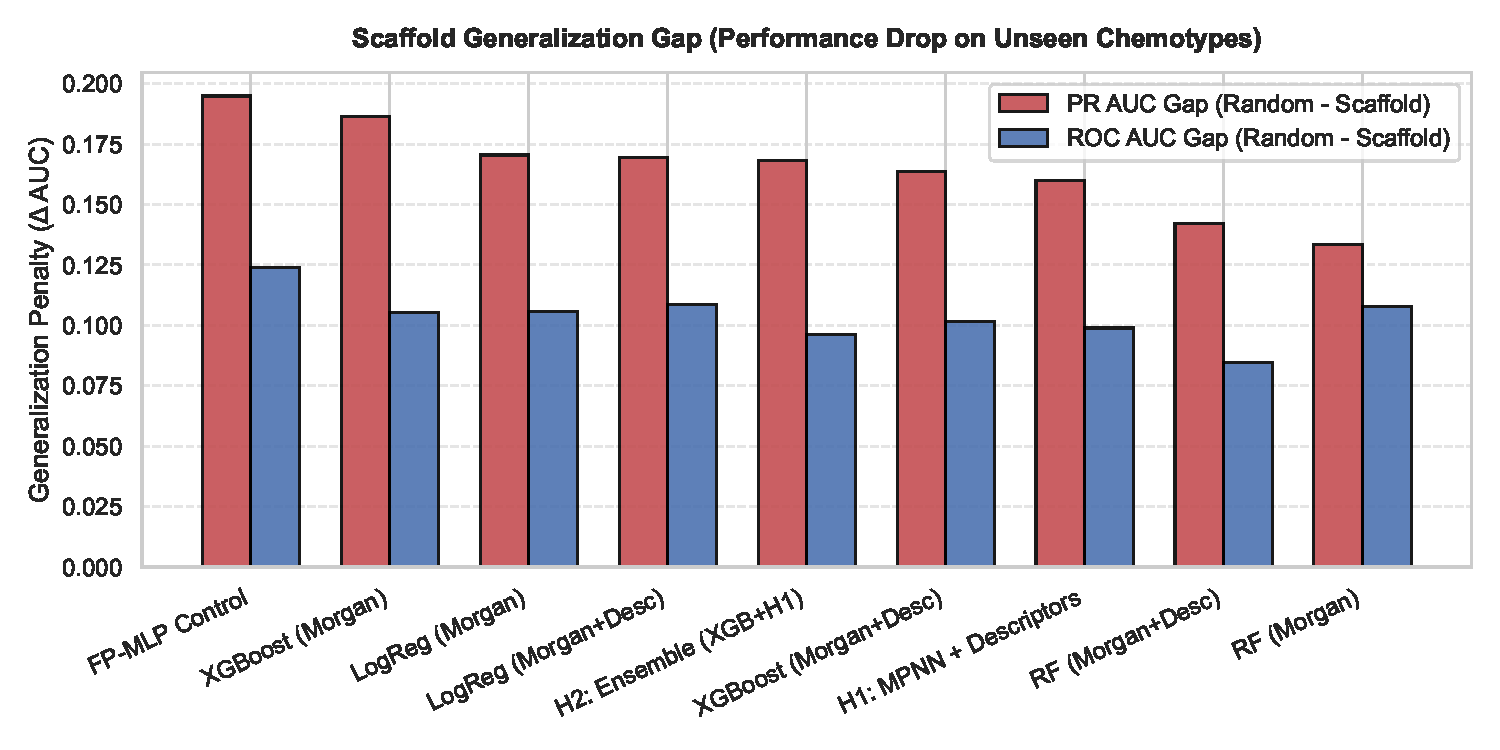
\includegraphics[width=0.48\textwidth]{figures/generalization_gap.pdf}
\caption{Chemical generalization penalty ($\Delta \text{AUC} = \text{Random} - \text{Scaffold}$) quantifying performance degradation on unseen molecular frameworks.}
\label{fig:gap}
\end{figure}

\subsection{Chemical Generalization Gap}
Figure~\ref{fig:gap} plots the performance drop observed when transitioning from random to scaffold evaluation. Every model experiences a large generalization penalty ($\Delta\text{PR} \approx 0.160$--$0.195$ and $\Delta\text{ROC} \approx 0.085$--$0.124$). 

Notably, the FP-MLP exhibits the largest PR~AUC generalization drop ($\Delta\text{PR} = 0.1949$), reflecting the tendency of dense networks to overfit fixed fingerprint bit patterns. In contrast, the H1 graph hybrid demonstrates superior scaffold robustness ($\Delta\text{PR} = 0.1600$), confirming that learned message passing features transfer better across scaffold shifts than memorized fingerprint fragments.

\begin{table}[htbp]
\centering
\caption{Ablation Suite on H1 Architecture (Scaffold Split, 3 Seeds)}
\label{tab:ablations}
\begin{tabular}{llcc}
\toprule
\textbf{Configuration} & \textbf{Description / Modification} & \textbf{PR AUC} & \textbf{ROC AUC} \\
\midrule
\textbf{Reference H1} & MPNN + 2D RDKit Descriptors & $\mathbf{0.3553}$ & $\mathbf{0.7384}$ \\
Ablation A6c & MPNN + Morgan + Descriptors (\texttt{both}) & $0.3309$ & $0.7186$ \\
Ablation A6b & MPNN + Morgan Fingerprints (\texttt{morgan}) & $0.2614$ & $0.6699$ \\
\textbf{Ablation A6a} & \textbf{Shuffled Descriptors (Negative Control)} & $\mathbf{0.2547}$ & $\mathbf{0.6951}$ \\
\bottomrule
\end{tabular}
\end{table}

\begin{figure}[htbp]
\centering
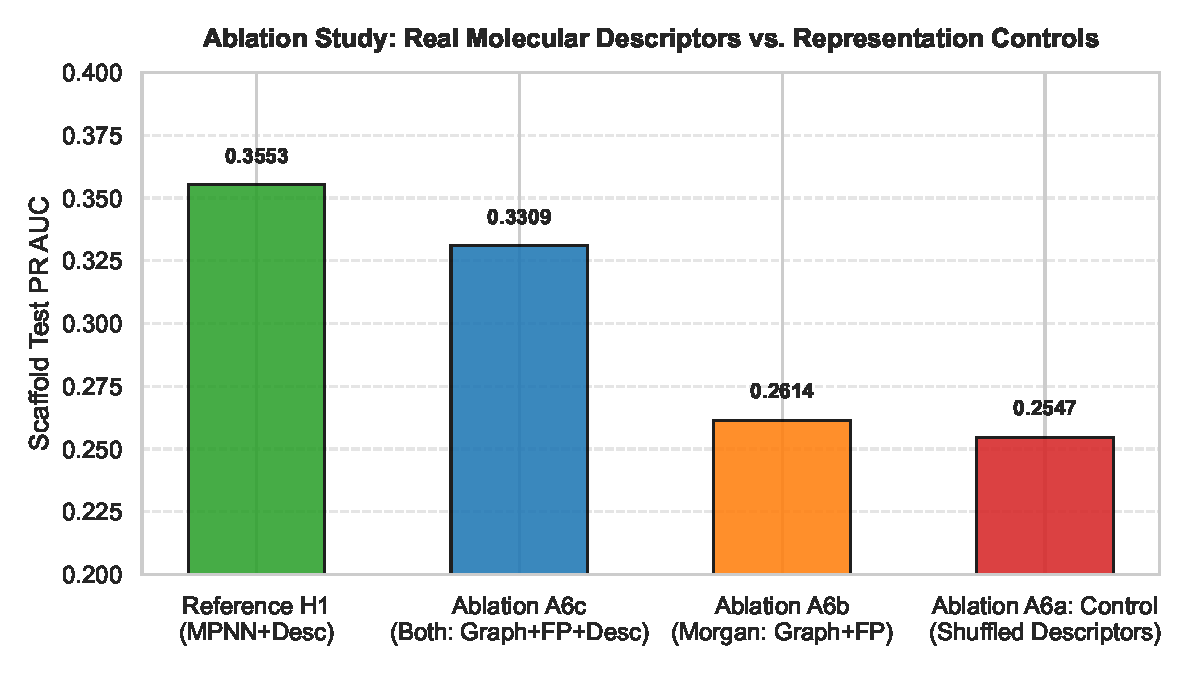
\includegraphics[width=0.45\textwidth]{figures/ablation_study.pdf}
\caption{Impact of input representations and negative controls on scaffold test PR~AUC.}
\label{fig:ablation_fig}
\end{figure}

\subsection{Ablation Suite and Negative Control Verification}
Table~\ref{tab:ablations} and Figure~\ref{fig:ablation_fig} detail the results of the ablation suite:
\begin{itemize}
    \item \textbf{Shuffled-Descriptor Control (\texttt{shuffled\_desc}):} When descriptor rows are permuted across molecules, performance crashes from $0.3553$ to $0.2547$ ($-0.1006$ PR~AUC; a $28.3\%$ collapse). This decisively refutes the hypothesis that hybrid gains are caused by parameter capacity or unspecific regularization.
    \item \textbf{Representation Substitution (\texttt{morgan}):} Replacing continuous descriptors with sparse 2,048-bit Morgan fingerprints drops PR~AUC to $0.2614$, proving that high-dimensional sparse vectors introduce severe optimization interference in deep graph architectures.
\end{itemize}

\begin{figure}[htbp]
\centering
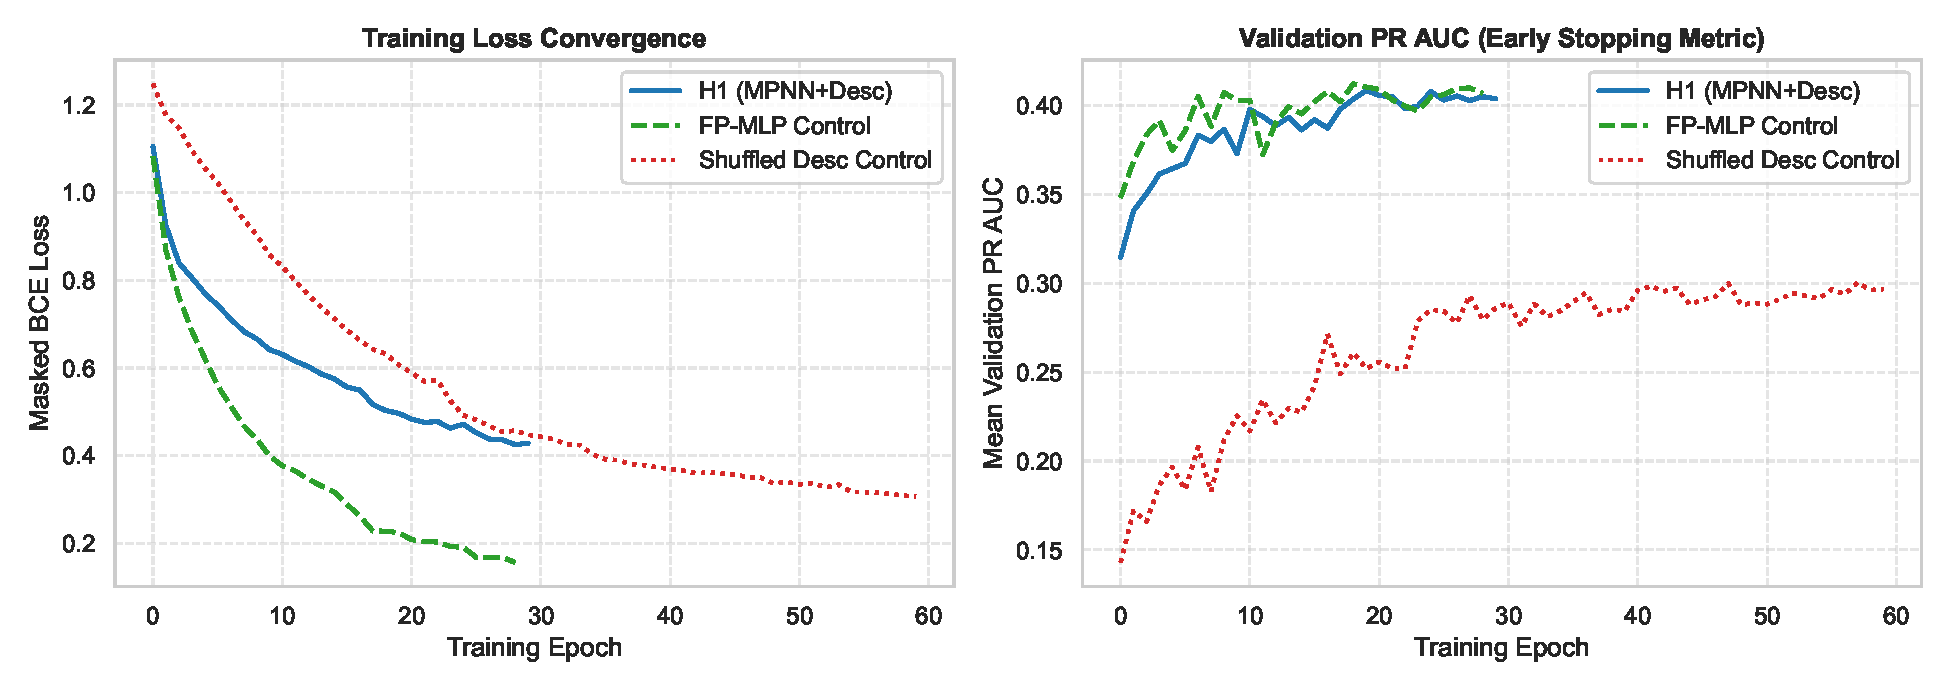
\includegraphics[width=0.48\textwidth]{figures/dl_learning_curves.pdf}
\caption{Training loss convergence and validation PR~AUC trajectory across training epochs.}
\label{fig:curves}
\end{figure}

\subsection{Optimization Dynamics and Learning Curves}
Figure~\ref{fig:curves} illustrates the training trajectories. Masked BCE loss decreases smoothly for H1, reaching optimal validation PR~AUC at epoch 19 ($0.4085$) before triggering early stopping restoration. The shuffled-descriptor control exhibits slower loss descent and lower plateau validation PR~AUC, confirming impaired learning dynamics.

\section{Architecture Ablations}
\label{sec:malhar-architecture-ablations}

We evaluated predeclared architecture changes to the frozen graph MPNN on the scaffold split with seeds 0--2. The base configuration uses hidden size 64, three message-passing steps, dropout 0.2, learning rate $10^{-3}$, and weight decay $10^{-5}$. Each run changes one architecture property: message-passing depth, bond features, or graph readout. For each seed, endpoint ROC AUC and PR AUC are averaged over the 12 tasks; the table reports the mean and sample standard deviation across the three seed-level means. The values come from \texttt{results/dl\_ablation\_test\_malhar.csv}.

\begin{table*}[t]
\centering
\caption{MPNN architecture ablations on the scaffold test split. Values are mean endpoint AUC $\pm$ sample SD across seeds 0--2.}
\label{tab:malhar-architecture-ablations}
\small
\begin{tabular}{lcc}
\toprule
Variant & PR AUC & ROC AUC \\
\midrule
A1: depth 1 & $0.2846 \pm 0.0129$ & $0.7388 \pm 0.0107$ \\
A2: depth 2 & $0.3007 \pm 0.0071$ & $0.7353 \pm 0.0096$ \\
A3: no bonds & $0.2947 \pm 0.0437$ & $0.7439 \pm 0.0187$ \\
P2: depth 4 & $0.2818 \pm 0.0172$ & $0.7311 \pm 0.0153$ \\
P2: sum readout & $0.3125 \pm 0.0172$ & $0.7586 \pm 0.0156$ \\
P2: mean readout & $0.3001 \pm 0.0043$ & $0.7391 \pm 0.0019$ \\
C1: shuffled labels & $0.1382 \pm 0.0063$ & $0.5305 \pm 0.0302$ \\
\bottomrule
\end{tabular}
\end{table*}

The shuffled-label control permuted complete training-label rows across molecules while leaving validation and test labels unchanged. Its seed-level mean test ROC AUCs were 0.5038, 0.5246, and 0.5632. The three-seed mean is 0.5305, but seed 2 exceeds the predeclared 0.55 threshold and warrants a leakage investigation.

\section{Technical Validation}
\label{sec:validation}

This section lists only checks that can be re-run from the repository.

\paragraph{Configuration freeze.}
The deep-learning configurations were frozen in commit \texttt{0aebd87}, whose only change is \texttt{results/best\_configs\_dl.json}; the deep-learning test-result files were committed afterwards. The Makefile target \texttt{dl-guard}, on which \texttt{dl-final}, \texttt{dl-ablate} and \texttt{dl-ensemble} depend, stops unless that file exists, is tracked and is identical to the committed version, and it prints that the configurations are frozen. The final and ablation modes of \texttt{src.dl.run} also exit unless the file exists. The commit history shows what was committed; it cannot show that no test evaluation was run locally before the freeze.

\paragraph{Alignment and leakage tests.}
\texttt{make phase2-test} runs four test files with \texttt{python -m pytest}; all 24 tests passed in our run.
\begin{itemize}
    \item \texttt{test\_graph\_alignment.py}: graph $i$ is row $i$ of the clean CSV (7,709 graphs), with identical labels and NaN pattern; split subsets keep row order and labels on both splits; atom counts match RDKit on 200 sampled molecules.
    \item \texttt{test\_extra\_alignment.py}: the Morgan-plus-descriptor rows (2,261 columns) follow the graphs in split order on both splits; the features are finite and roughly standardized on the training rows.
    \item \texttt{test\_gate0\_ranajeet.py}: row counts agree across the CSV, graphs and feature arrays; sampled SMILES, atom counts, labels and stored Morgan fingerprints match the CSV; the preprocessed descriptors have 213 columns; the scaffold split covers all rows without overlap; \texttt{attach\_extra} keeps row order, and shuffling the rows breaks it (negative control).
    \item \texttt{test\_dl\_smoke.py}: the masked loss ignores missing labels and \texttt{mask\_missing=False} treats them as negatives; the positive weight is $n_{\text{neg}}/n_{\text{pos}}$ per endpoint with the cap; model output shapes, invariance to atom order, early stopping that restores the best weights, and reproducibility for a fixed seed.
\end{itemize}
The Phase~1 suite adds a check that no scaffold group spans two partitions and that the empty scaffold stays in one partition (\texttt{test\_splits.py}), that transforming new data leaves fitted descriptor statistics unchanged (\texttt{test\_features.py}), and that missing labels are excluded rather than filled with zero (\texttt{test\_evaluate.py}).

\paragraph{Scaffold split and predictions.}
The scaffold split has 6,167 training, 771 validation and 771 test molecules. Of the 7,709 molecules, 1,753 are acyclic and share the empty scaffold; all are in training, none in validation or test, so scaffold validation and test contain only ring-containing molecules. All 30 saved test-prediction files for XGBoost, FP-MLP, GCN, MPNN and H1 (both splits, seeds 0--2) have shape $771 \times 12$, contain only finite values, and reproduce the committed per-endpoint ROC and PR~AUC when re-scored against the test labels from the split file.

\paragraph{Controls.}
With descriptor rows permuted across molecules (same architecture and parameter count), H1's scaffold test PR~AUC falls from $0.3553$ to $0.2547$ (ROC~AUC $0.6951$), so its benefit depends on correct alignment between molecules and descriptor values. In the shuffled-label control, training labels are permuted across molecules and the MPNN is evaluated on unchanged test labels. Its test ROC~AUC is $0.5038$, $0.5246$ and $0.5632$ for seeds 0, 1 and 2 (mean $0.5305$, mean PR~AUC $0.1382$). Seed 2 is above the $0.55$ threshold set for this control. We have not investigated the cause, and averaging over seeds does not remove the warning.

\section{Discussion and Limitations}
\label{sec:discussion}

\subsection{When Does Deep Learning Help, and When Does It Not?}
We compare classical machine learning on engineered descriptors with deep learning on molecular graphs and report what the results do and do not support.

\textbf{1. Graph structure versus flat inputs: weak evidence.} The H1 hybrid (\texttt{mpnn+desc}) has a higher observed mean scaffold PR~AUC than the FP-MLP control ($0.3553$ vs.\ $0.3429$, $+0.0124$) and a higher PR~AUC on 9 of 12 endpoints, largest on \texttt{NR-Aromatase} ($+0.0980$), but the paired Wilcoxon test gives $p = 0.1514$, so the difference is not significant. The two models also differ in their inputs (the FP-MLP sees Morgan bits plus descriptors, H1 sees the graph plus descriptors). The graph-only models score below the FP-MLP in mean scaffold PR~AUC (GCN $0.3397$, MPNN $0.3069$).

\textbf{2. The GCN beat the plain MPNN.} The GCN scores higher than the MPNN on scaffold ($0.3397$ vs.\ $0.3069$ PR~AUC), with a higher PR~AUC on 11 of 12 endpoints (mean difference $+0.0328$, $p = 0.0015$), and has a smaller seed standard deviation ($0.0027$ vs.\ $0.0180$). The more expressive edge-network MPNN therefore did not improve on the simpler baseline here; we did not investigate why.

\textbf{3. Classical tree ensembles remain best on scaffold.} Random Forest ($0.4035$ PR~AUC) and XGBoost ($0.4010$) on combined fingerprints and descriptors score above every deep model and above both H2 variants on the scaffold split. This is in line with the comparison study of Jiang et al.~\cite{jiang2021could}, who report that descriptor-based models are often competitive with graph neural networks. On the random split the primary H2 has the highest mean PR~AUC ($0.5727$ vs.\ $0.5647$ for XGBoost), without a significant difference ($9/3$ endpoint wins, $p = 0.0923$).

\textbf{4. Descriptors as global information.} The frozen MPNN has $628{,}300$ trainable parameters (counted from the code with the frozen configuration) and is trained on about $6{,}200$ molecules. Descriptors such as lipophilicity or polar surface area encode whole-molecule properties directly, which may help a model trained on little data; we did not test this explanation. What the shuffled-descriptor control shows is narrower: with the same architecture, permuting descriptor rows across molecules lowers H1 from $0.3553$ to $0.2547$ PR~AUC, so its benefit depends on correct alignment between molecules and descriptor values. The control does not identify which descriptors matter or why.

\textbf{5. Ensembling.} The primary H2 (XGBoost plus FP-MLP, partner selected on validation PR~AUC) scores $0.3945$ on scaffold. It beats its deep components (against the FP-MLP on 12 of 12 endpoints, $p = 0.0005$; against H1 on 11 of 12, $p = 0.0093$) but not XGBoost alone: it wins on 4 endpoints and loses on 8 (mean difference $-0.0065$, $p = 0.5186$). With equal-weight rank averaging, fusing a deep model with XGBoost therefore did not improve on XGBoost alone on the scaffold split. We did not test other fusion weights, and we make no claim about error complementarity.

\subsection{Methodological Limitations}
Our protocol freezes the configurations before test results are committed, but several limitations remain:

\begin{itemize}
    \item \textbf{Small Dataset Size and Single Benchmark:} Our experiments are conducted exclusively on the Tox21 benchmark ($N = 7,709$). In massive screening libraries ($N > 100,000$) or under self-supervised pre-training regimes, deep graph architectures typically exhibit stronger scaling advantages that cannot be realized on small datasets.
    \item \textbf{Endpoint Sample Size and Statistical Power:} With $K = 12$ endpoints, non-parametric statistical tests (such as the Wilcoxon signed-rank test) possess inherently limited statistical power. Bootstrap intervals on the seed-0 predictions exclude zero on only 1 of 12 endpoints for H1 minus FP-MLP, so endpoint-level evidence is weaker than the pooled win counts. More assays would give tighter bounds.
    \item \textbf{Hyperparameter Budget Constraints:} Hyperparameter search was limited to at most 8 configurations per model, each evaluated once with seed 0 on the scaffold validation split, and the scaffold choice is reused unchanged on the random split. H1 has no search of its own: it reuses the frozen MPNN configuration. A larger search might change the ranking of the deep models.
    \item \textbf{Ablations run on the test split.} The ablations were evaluated on the test split, so they are explanatory and were not used to choose any configuration. The command lines of the ablation runs are not recorded in the repository and were reconstructed from the result files. In the shuffled-label control (Section~\ref{sec:malhar-architecture-ablations}) the seed-2 test ROC~AUC ($0.5632$) is above the predeclared $0.55$ threshold; the cause has not been investigated.
    \item \textbf{2D Topological Graphs vs.\ 3D Conformers:} Our graph formulation is restricted to 2D topological connectivity and atom/bond features. Toxicity bioassays frequently depend on 3D stereochemical fit into biological receptor binding pockets (e.g., nuclear receptor ligand binding domains). Incorporating 3D conformer ensembles or quantum chemical surface potentials represents an open technical frontier.
\end{itemize}

\section{Conclusion}
\label{sec:conclusion}

In this Phase~2 investigation we compared deep and hybrid models against the Phase~1 tree baselines on Tox21 under one frozen-configuration protocol (Phase~1 scaffold and random splits, three seeds). The evidence supports four conclusions, with the limits stated:
\begin{enumerate}
    \item \textbf{Tree models remain best on scaffold.} Random Forest ($0.4035$ PR~AUC) and XGBoost ($0.4010$) on Morgan fingerprints plus descriptors score above every deep model (H1 $0.3553$, FP-MLP $0.3429$, GCN $0.3397$, MPNN $0.3069$) and above both H2 variants.
    \item \textbf{Among the deep models.} The GCN scores higher than the plain MPNN ($11$ of $12$ endpoints, $p = 0.0015$). H1 has a higher observed mean PR~AUC than the FP-MLP ($+0.0124$, $9$ of $12$ endpoints), but the difference is not significant ($p = 0.151$).
    \item \textbf{Descriptor alignment matters for H1.} Permuting the descriptor rows across molecules lowers H1 from $0.3553$ to $0.2547$ PR~AUC, so its benefit depends on correct molecule--descriptor alignment. The experiment does not identify the mechanism.
    \item \textbf{Equal-weight rank fusion did not beat XGBoost on scaffold.} H2 (XGBoost plus the FP-MLP, selected on validation PR~AUC; $0.3945$) beats both of its deep components but not XGBoost alone ($4$ wins and $8$ losses, $p = 0.5186$). On the random split it is nominally ahead ($0.5727$ vs.\ $0.5647$) without significance ($p = 0.0923$).
\end{enumerate}

These conclusions rest on one dataset, one fixed split of each type, three seeds and 12 endpoints, so the tests have low power. In this benchmark, descriptor-based tree models remain the strongest single models, and the deep models and the ensemble did not surpass them on the scaffold split.


\bibliographystyle{IEEEtran}
\bibliography{references_dl}

\end{document}
